%% LyX 2.3.6 created this file.  For more info, see http://www.lyx.org/.
%% Do not edit unless you really know what you are doing.
\documentclass[english]{article}
\usepackage[T1]{fontenc}
\usepackage[latin9]{inputenc}
\usepackage{float}
\usepackage{graphicx}

\makeatletter

%%%%%%%%%%%%%%%%%%%%%%%%%%%%%% LyX specific LaTeX commands.
%% Because html converters don't know tabularnewline
\providecommand{\tabularnewline}{\\}
\floatstyle{ruled}
\newfloat{algorithm}{tbp}{loa}
\providecommand{\algorithmname}{Algorithm}
\floatname{algorithm}{\protect\algorithmname}

\makeatother

\usepackage{babel}
\begin{document}
\title{MinCenter: using clustering in global optimization}
\author{Vasileios Charilogis, Ioannis G. Tsoulos\thanks{Corresponding author. Email: itsoulos@uoi.gr}}
\date{Department of Informatics and Telecommunications, University of Ioannina,
Greece}
\maketitle
\begin{abstract}
A common problem arises in many scientific fields is that of locating
the global minimum of a multimodal function. A novel clustering technique
that tackles this problem is introduced here. The proposed method
creates clusters from uniform samples of the objective function with
the usage of the Kmeans clustering technique. For every cluster a
center is created. Finally, a simple rejection procedure is applied
to the created clusters in order to remove clusters that are close
to others. The proposed method is tested on a series of well - known
optimization problems from the relevant literature and the results
are reported and compared against the simple Multistart global optimization
method.
\end{abstract}
\textbf{Keywords}: Global optimization, clustering, hubrid methods,
numerical methods.

\section{Introduction }

A novel method that estimates the global minimum of a continuous and
differentiable function $f:S\rightarrow R,S\subset R^{n}$ is proposed
in the current article. The global optimum location problem is usually
defined as: 
\begin{equation}
x^{*}=\mbox{arg}\min_{x\in S}f(x)\label{eq:eq1}
\end{equation}
where $S$ is 
\[
S=\left[a_{1},b_{1}\right]\otimes\left[a_{2},b_{2}\right]\otimes\ldots\left[a_{n},b_{n}\right]
\]
A review of the recent advantages in the area of the Global Optimization
can be found in \cite{global_review}. Methods that discover the global
minimum can be used in many areas such as: economics \cite{global_econ1,global_econ2},
physics \cite{global_physics1,global_physics2}, chemistry \cite{global_chemistry1,global_chemistry2},
medicine \cite{global_med1,global_med2} etc. Global optimization
methods usually are divided into two main categories: deterministic
and random search methods. Common methods of the first category are
the so called Interval methods \cite{interval1,interval2}, where
the set $S$ is divided iteratively in subregions using some criteria.
On the other hand, random search methods are used in the majority
of cases, because they can be implement easy and they do not depend
on a some a priori information about the objective function. A small
set of random search methods may include Controlled Random Search
methods \cite{crs1,crs2,crs3}, Simulated Annealing methods \cite{simann1,simann2},
Differential Evolution methods \cite{diffe1,diffe2}, Particle Swarm
Optimization methods \cite{pso1,pso2}, Ant Colony Optimization \cite{aco1,aco2},
Genetic algorithms \cite{ga1,ga2,ga3} etc. 

A subclass of random search methods are the clustering techniques
as proposed by Rinnooy Kan \cite{kan_clusterin}, Ali \cite{ali_cluster},
Tsoulos \cite{minfinder}, etc. These methods are try to estimate
the clusters of function in order to minimize the effort required
to compute the global minimum or all the local minima of the function.
The term cluster refers to a set of points that are believed, under
some asymptotic considerations, to belong to the same region of attraction
of the function. The region of attraction for a local minimum $x^{*}$
is defined as:
\begin{equation}
A\left(x^{*}\right)=\left\{ x:\ x\in S\subset R^{n},\ L(x)=x^{*}\right\} 
\end{equation}
 where $L(x)$ is a local search procedure that starts from a given
point $x$ and terminates when a local minimum is discovered. Common
local search procedures are BFGS\cite{bfgs,powell}, Steepest Descent\cite{steepest},
L-Bfgs \cite{lbfgs} for large scaled functions etc. 

The proposed method creates clusters iteratively using the well -
known technique of the K-Means clustering introduced by MacQueen\cite{kmeans}.
For every cluster a representative is constructed using the K-means
method and afterwards a rejection procedure is utilized in order to
reduce the number of representatives. Finally, for every remain point
a local search procedure is started to locate the global minimum of
the function.

The rest of this article is organized as follows: in section \ref{sec:Method-description}
the proposed method is described in detail, in section \ref{sec:Experiments}
some experimental test functions from the relevant literature are
described and a series of test are performed on those functions and
finally in section \ref{sec:Conclusions} some conclusions are discussed
as well as some guidelines to improve the proposed method.

\section{Method description \label{sec:Method-description}}

The proposed method is initially based on the commonly used global
optimization method named Multistart. The proposed method creates
clusters from the objective function. The multistart method is one
of the simplest global optimization technique which start a local
search optimizer such as BFGS from different random points and yields
the lowest discovered minimum as the global one. As it was demonstrated
by various researchers \cite{stop1,stop2}, if the number of local
minimum is finite then Multistart method is capable to locate the
global minimum. 

Due to its simplicity, the Multistart method is the base method for
a series of stochastic methods in the relevant literature such as
hybrid methods\cite{mshybrid1,mshybrid2}, GRASP methods\cite{grasp}
etc. Also, it has been tested on many practical problems such as the
TSP problem \cite{multistart-tsp}, the vehicle routing problem \cite{multistart-vehicle},
the maximum clique problem \cite{multistart-clique}, flowshop rescheduling
\cite{multistart-res}, energy consumption etc. The base method has
been extended in different works such as enhanced stopping rules for
the multistart method \cite{stop1,stop2,stop3,stop4}, parallel techniques
\cite{parallel-multistart,parallel-multistart2}, multistart hybrid
methods executed on modern GPU architectures \cite{msgpu1,msgpu2}
etc. Also, a variety of methods have been introduced that enhance
the sampling in the procedure such as the repulsion sampling \cite{mssampling1},
methods where the sampling is guided by a neural network \cite{mssampling2}
etc. Furthermore, the multistart method has been extended to solve
also constrained optimization problems \cite{mscons1}. 

The main steps of a typical Multistart procedure are shown in Algorithm
\ref{fig:The-main-steps}.

\begin{algorithm}
\caption{The main steps of the Multistart method.\label{fig:The-main-steps}}

\begin{enumerate}
\item \textbf{Initialization} step.
\begin{enumerate}
\item \textbf{Set} \textbf{$M$ }as the total number of samples.
\item \textbf{Set} $\left(x^{*},y^{*}\right)$ as the global minimum. Initialize
$y^{*}$ to a very large value.
\end{enumerate}
\item \textbf{Sampling} step.
\begin{enumerate}
\item \textbf{For} $i=1\ldots M$ \textbf{Do}
\begin{enumerate}
\item \textbf{Sample} a point $x_{i}\in S$
\item $y_{i}=\mbox{LS}\left(x_{i}\right)$. Where LS(x) is a local search
procedure.
\item \textbf{If} $y_{i}\le y^{*}$ then $x^{*}=x_{i},y^{*}=y_{i}$
\end{enumerate}
\item \textbf{EndFor}
\end{enumerate}
\end{enumerate}
\end{algorithm}

The proposed method replaces the sampling step of the Multistart method
with the usage of centroids constructed by Kmeans clustering. The
main steps of the Kmeans method are given in Algorithm \ref{fig:The-algorithm-Kmeans.}.
The estimated centroids are iteratively enhanced with Kmeans and new
samples that added each time for a predefined number of times. Having
created the centroids a rejection procedure is applied to reduce the
number of centroids. The rejection procedure removes from the set
of centers, points that have many neighbors in a predefined radius.
The rejection procedure is necessary to remove from the set samples,
that possible will yeld the same local optimum after the application
of the local search procedure. The proposed method is described in
Algorithm \ref{fig:The-proposed-method.}.

\begin{algorithm}
\caption{The algorithm Kmeans.\label{fig:The-algorithm-Kmeans.}}

\begin{enumerate}
\item \textbf{Repeat}
\begin{enumerate}
\item $S_{j}=\left\{ \right\} ,\ j=1..K$
\item \textbf{For} every sample $x_{i}$ \textbf{Do}
\begin{enumerate}
\item \textbf{Set} $j^{*}=\min_{i=1}^{K}\left\{ D\left(x_{i},c_{j}\right)\right\} $,
where $j^{*}$ is the nearest center for sample $x_{i}$. 
\item \textbf{Set} $S_{j^{*}}=S_{j^{*}}\cup\left\{ x_{i}\right\} $.
\end{enumerate}
\item \textbf{EndFor}
\item \textbf{For} every center $c_{j}$ \textbf{Do}
\begin{enumerate}
\item \textbf{Set} $M_{j}$=number of elements in $S_{j}$
\item \textbf{Update} $c_{j}$
\[
c_{j}=\frac{1}{M_{j}}\sum_{i=1}^{M_{j}}x_{i}
\]
\end{enumerate}
\item \textbf{EndFor} 
\end{enumerate}
\item \textbf{Terminate} when $c_{j}$ no longer change.
\end{enumerate}
\end{algorithm}
\begin{algorithm}
\caption{The proposed method.\label{fig:The-proposed-method.}}

\begin{enumerate}
\item \textbf{Initialization} step.
\begin{enumerate}
\item \textbf{Set} $M$ as the number of samples.
\item \textbf{Set} $\left(x^{*},y^{*}\right)$ as the global minimum. Initialize
$y^{*}$ to a very large value.
\item \textbf{Set }$K$ the number of teams, where $K<M$.
\item \textbf{Set} $K_{\mbox{MAX}}$ the number of construction iterations
for the KMeans algorithm.
\item \textbf{Set} $C=\left\{ \right\} $, as the set of constructed centers.
\end{enumerate}
\item \textbf{Construction} step.
\begin{enumerate}
\item \textbf{For} $i=1..K_{\mbox{MAX}}$ \textbf{Do}
\begin{enumerate}
\item \textbf{Sample} $M$ points from the objective function $S=\left\{ x_{1},x_{2},\ldots,x_{M}\right\} $
\item \textbf{Update} the centers $C$ with the set $S$, using Kmeans.
\end{enumerate}
\item \textbf{EndFor}
\end{enumerate}
\item \textbf{Create} the set $R$ from $C$ using the rejection algorithm
of Algorithm \ref{fig:The-rejection-mechanism.}.
\item \textbf{Evaluation} step.
\begin{enumerate}
\item \textbf{For} $i=1\ldots\left|R\right|$ \textbf{Do}
\begin{enumerate}
\item \textbf{Set} $x_{i}=R_{i}$
\item $y_{i}=\mbox{LS}\left(x_{i}\right)$. Where LS(x) is a local search
procedure.
\item \textbf{If} $y_{i}\le y^{*}$ then $x^{*}=x_{i},y^{*}=y_{i}$
\end{enumerate}
\item \textbf{EndFor}
\end{enumerate}
\end{enumerate}
\end{algorithm}
\begin{algorithm}
\caption{The rejection algorithm.\label{fig:The-rejection-mechanism.}}

\begin{enumerate}
\item \textbf{Set} $C$ the set of centers.
\item \textbf{Set} $R=\emptyset$ the outcome of the rejection algorithm.
\item \textbf{Set} $D_{\mbox{min}}=\min_{i\ne j}\left\Vert c_{i}-c_{j}\right\Vert $
\item \textbf{Set} $F>1$, a double value.
\item \textbf{Set} $N_{\mbox{min}}>1$, an integer value.
\item \textbf{For} every center $c_{i}$ \textbf{Do}
\begin{enumerate}
\item \textbf{Set} $N=0$
\item \textbf{For} every center $c_{j},\ i\ne j$ \textbf{Do}
\begin{enumerate}
\item \textbf{If} $\left\Vert c_{i}-c_{j}\right\Vert \le FD_{\mbox{\mbox{min}}}$
\textbf{then} $\ N=N+1$
\end{enumerate}
\item \textbf{EndFor}
\item \textbf{If} $N<N_{\mbox{min}}\ $ \textbf{then} $R=R\cup c_{i}$
\end{enumerate}
\item \textbf{EndFor}
\item \textbf{Return} $R$
\end{enumerate}
\end{algorithm}


\section{Experiments \label{sec:Experiments}}

\subsection{Test functions }

In order to measure the effectiveness of the proposed approach we
utilize several benchmark functions from the relevant literature \cite{Ali1,Floudas1}.
The names and the complete forms of these equations can be obtained
from \cite{mssampling2}.

\subsection{Experimental Results}

The proposed method was tested against the traditional multistart
global optimization method on the series of benchmark problems. The
parameters used in the conducted experiments are listed in Table \ref{tab:The-values-for}.
The method was coded using the OpenMP library\cite{openmp} in order
to take advantage of multi - core modern computing systems and the
experiments were conducted on a cluster of systems running the Linux
operating system. The results from the experiments are listed in Tables
\ref{tab:Multistart-results.} and \ref{tab:The-proposed-method.}.
The methods were executed 30 times for each test function and averages
were measured. In every run different seed for the random generator
(drand48() function of C) was used. The numbers appeared in the parentheses
stand for the percentage of runs where the global minimum was located
sucessfully and they are not shown if the success was 100\%. The last
row represents the total number of function calls. The local search
procedure used (denotes as LS(x)) was a BFGS variant due to Powell\cite{powell}.

In Table \ref{tab:Multistart-results.} the results for the Multistart
global optimization procedure are shown. The column $M=100$ denotes
the application of the algorithm given in Algorithm \ref{fig:The-main-steps}
with $M=100$ samples. The column $M=200$ stands for the Multistart
algorithm using 200 samples. The last column stands for the results
of the Multistart method with 100 samples and the application of the
proposed rejection procedure of algorithm in Algorithm \ref{fig:The-rejection-mechanism.}
in the samples before the application of the local search procedure.
It is evident that the application of the rejection procedure does
not reduce significantly the number of function calls for the multistart
case.

In Table \ref{tab:The-proposed-method.} the experimental results
for the proposed method are listed. The column $M=100$ stands for
the usage of 100 samples in the proposed method (parameter $M$) and
the column $M=200$ for 200 samples. The proposed method has significantly
lower number of function calls than the Multistart method and as the
number of samples increases (parameter $M$) the method requires lower
amount of function calls to estimate the global minimum. This means
that the method tends to create more accurate clusters (clusters that
emulate the true regions of attraction) of the objective function
as the number of samples increases. To fully demonstrate it an additional
run has been performed using different values for the samples and
constant number of centers: in Figure \ref{fig:Plot-for-the} the
number of required function calls for Function EXP4 are plotted against
the number of samples. The number of samples varies between 100 and
900 and the number of centers remains $K=100$ for all the runs. As
is is evident, the number of function calls remains constant, regarding
the increase of samples. Also, to compare the proposed method with
M=100 with the M=200 for different functions, the Wilcoxon signed-rank
test was used. The results obtained with this statistical test are
shown in Figure \ref{fig:Statistical-comparisons-for}.

\begin{table}
\caption{The values for the parameters used in the conducted experiments.\label{tab:The-values-for}}

\centering{}%
\begin{tabular}{|c|c|}
\hline 
PARAMETER & VALUE\tabularnewline
\hline 
\hline 
$K$ & 100\tabularnewline
\hline 
$K_{\mbox{max}}$ & 100\tabularnewline
\hline 
$F$ & 1.5\tabularnewline
\hline 
$N_{\mbox{min}}$ & 3\tabularnewline
\hline 
\end{tabular}
\end{table}

\begin{table}
\caption{Multistart results.\label{tab:Multistart-results.}}

\centering{}%
\begin{tabular}{|c|c|c|c|}
\hline 
Function & $M=100$ & $M=200$ & $M=100,$Rejection\tabularnewline
\hline 
\hline 
B2 & 4518 & 8849 & 4472\tabularnewline
\hline 
Easom & 943 & 1949 & 933\tabularnewline
\hline 
Bf1 & 4508 & 9300 & 4469\tabularnewline
\hline 
Bf2 & 3750 & 7621 & 3666\tabularnewline
\hline 
Branin & 1948 & 3855 & 1938\tabularnewline
\hline 
Camel & 2669 & 4983 & 2502\tabularnewline
\hline 
CM4 & 5714 & 11783 & 5644\tabularnewline
\hline 
CM8 & 7341(0.33) & 14813(0.60) & 7289(0.33)\tabularnewline
\hline 
DIFFPOWER10 & 123729 & 248924 & 121012\tabularnewline
\hline 
ELP4 & 1203 & 2474 & 1158\tabularnewline
\hline 
ELP8 & 1721 & 3395 & 1652\tabularnewline
\hline 
ELP16 & 2789 & 5485 & 2252\tabularnewline
\hline 
EXP4 & 3646 & 7063 & 3609\tabularnewline
\hline 
EXP8 & 3723 & 7447 & 3651\tabularnewline
\hline 
EXP16 & 3835 & 7486 & 3310\tabularnewline
\hline 
GKLS250 & 1486 & 2928 & 1426\tabularnewline
\hline 
GKLS350 & 1030(0.97) & 2007 & 913(0.87)\tabularnewline
\hline 
GKLS3100 & 1020(0.77) & 2005 & 1018(0.77)\tabularnewline
\hline 
GRIEWANK2 & 3131(0.70) & 6197(0.97) & 3048(0.70)\tabularnewline
\hline 
GRIEWANK10 & 10449 & 20763 & 10226\tabularnewline
\hline 
HANSEN & 2482 & 4997 & 2422\tabularnewline
\hline 
HARTMAN3 & 2911 & 5753 & 2868\tabularnewline
\hline 
HARTMAN6 & 3825 & 7875 & 3787\tabularnewline
\hline 
POTENTIAL3 & 5237 & 10784 & 5178\tabularnewline
\hline 
POTENTIAL5 & 11594 & 22331 & 10127\tabularnewline
\hline 
POTENTIAL10 & 20361 & 40592 & 5089(0.70)\tabularnewline
\hline 
RASTRIGIN & 2345 & 4731 & 2242(0.93)\tabularnewline
\hline 
SHEKEL5 & 3852 & 7841 & 3730\tabularnewline
\hline 
SHEKEL7 & 3951 & 7149 & 3885\tabularnewline
\hline 
SHEKEL10 & 3982 & 6987 & 3890\tabularnewline
\hline 
SINU4 & 3317 & 6624 & 3246\tabularnewline
\hline 
SINU8 & 4883 & 10015 & 4791\tabularnewline
\hline 
SINU16 & 8731 & 17005 & 8692\tabularnewline
\hline 
TEST2n4 & 3258 & 6608 & 3216\tabularnewline
\hline 
TEST2n5 & 3565 & 7128 & 3534\tabularnewline
\hline 
TEST2n6 & 3804(0.90) & 7790 & 3850(0.90)\tabularnewline
\hline 
TEST2n7 & 4203(0.83) & 8501(0.97) & 4155(0.77)\tabularnewline
\hline 
\textbf{TOTAL} & \textbf{281454(0.93)} & \textbf{562038(0.98)} & \textbf{259160(0.92)}\tabularnewline
\hline 
\end{tabular}
\end{table}

\begin{table}
\caption{The proposed method with $K=100$ centers.\label{tab:The-proposed-method.}}

\begin{centering}
\begin{tabular}{|c|c|c|}
\hline 
Function & $M=100$ & $M=200$\tabularnewline
\hline 
\hline 
B2 & 4073 & 3886\tabularnewline
\hline 
Easom & 830 & 782\tabularnewline
\hline 
Bf1 & 4046 & 3864\tabularnewline
\hline 
Bf2 & 3346 & 3153\tabularnewline
\hline 
Branin & 1699 & 1623\tabularnewline
\hline 
Camel & 2338 & 2237\tabularnewline
\hline 
CM4 & 4434 & 4043\tabularnewline
\hline 
CM8 & 3084(0.63) & 1819(0.50)\tabularnewline
\hline 
DIFFPOWER10 & 26726 & 17980\tabularnewline
\hline 
ELP4 & 971 & 908\tabularnewline
\hline 
ELP8 & 601 & 338\tabularnewline
\hline 
ELP16 & 139 & 100\tabularnewline
\hline 
EXP4 & 2764 & 2522\tabularnewline
\hline 
EXP8 & 1564 & 943\tabularnewline
\hline 
EXP16 & 245 & 179\tabularnewline
\hline 
GKLS250 & 1337 & 1275\tabularnewline
\hline 
GKLS350 & 911(0.93) & 777(0.83)\tabularnewline
\hline 
GKLS3100 & 939(0.97) & 796(0.97)\tabularnewline
\hline 
GRIEWANK2 & 2812(0.77) & 2684(0.70)\tabularnewline
\hline 
GRIEWANK10 & 1812 & 1152(0.80)\tabularnewline
\hline 
HANSEN & 2210 & 2077\tabularnewline
\hline 
HARTMAN3 & 2400 & 1993\tabularnewline
\hline 
HARTMAN6 & 2707 & 2369\tabularnewline
\hline 
POTENTIAL3 & 1246 & 714\tabularnewline
\hline 
POTENTIAL5 & 752 & 664\tabularnewline
\hline 
POTENTIAL10 & 1621(0.23) & 1045(0.10)\tabularnewline
\hline 
RASTRIGIN & 2016 & 1917\tabularnewline
\hline 
SHEKEL5 & 3520 & 3116\tabularnewline
\hline 
SHEKEL7 & 3515 & 3113\tabularnewline
\hline 
SHEKEL10 & 3586 & 3237\tabularnewline
\hline 
SINU4 & 2548 & 2268\tabularnewline
\hline 
SINU8 & 2121 & 1624\tabularnewline
\hline 
SINU16 & 546 & 358\tabularnewline
\hline 
TEST2n4 & 2436 & 2198\tabularnewline
\hline 
TEST2n5 & 2186(0.97) & 1840(0.97)\tabularnewline
\hline 
TEST2n6 & 2648(0.80) & 2300(0.83)\tabularnewline
\hline 
TEST2n7 & 2469(0.77) & 2173(0.73)\tabularnewline
\hline 
\textbf{TOTAL} & \textbf{103198(0.95)} & \textbf{84067(0.93)}\tabularnewline
\hline 
\end{tabular}
\par\end{centering}
\end{table}

\begin{figure}

\caption{Plot for the EXP4 functions as the number of samples increases.\label{fig:Plot-for-the}}

\begin{centering}
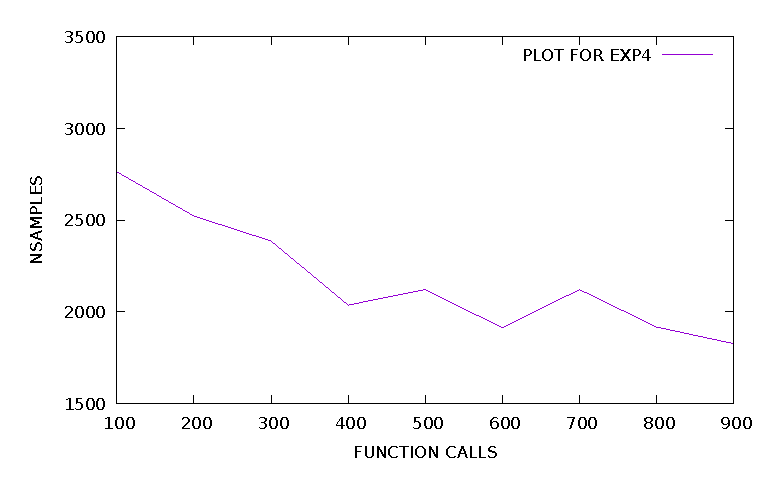
\includegraphics{exp4}
\par\end{centering}
\end{figure}

\begin{figure}
\caption{Scatter plot representation and Wilcoxon rank-sum test results of
the comparison between the samples M=100 with the M=200 for different
functions. A p-value of less than 0.05 (2-tailed) was used for statistical
significance.\label{fig:Statistical-comparisons-for}}

\centering{}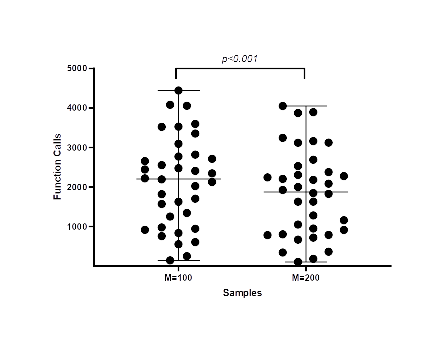
\includegraphics[scale=1.2]{statistics_mincenter}
\end{figure}


\section{Conclusions \label{sec:Conclusions}}

A new clustering method was introduced in this article to tackle to
global optimization problem. For every cluster gradually a representative
is created using the well - known Kmeans method. Afterwards, the clusters
are reduced in number using a simple rejection procedure. The proposed
method was tested on a series of benchmark problems from the relevant
literature and it is compared against the Multistart method and the
results are reported. The proposed method outperforms traditional
multistart due to creation of the centers, that seem to be more accurate
representatives of the regions of attractions for the underlying function.
To achieve better representation of these regions of attractions,
the centers are gradually improved through repetitive sampling of
the objective function. 

Despite the promising results, the method has some limitations that
can be addressed in future research. First of all the method depends
heavily on the Kmeans algorithm. The method creates $K$ clusters
that are enhanced through sampling, but this processes can take long
especially for problems of higher dimension. A possible solution could
be to use parallel techniques for the estimation of the clusters.
Also, the method requires an excessive memory storage just to hold
the member points for the $K$ clusters and some efficient memory
allocation mechanism should be incorporated here.

Judging from the reported results, the proposed method seems to be
very promising and a series of enhancements could be applied on the
method such as:
\begin{enumerate}
\item Dynamic selection of K in Kmeans algorithm. 
\item Better estimation of the critical distance between clusters in the
rejection procedure.
\item Usage of more efficient stopping rules to prevent the method from
unnecessary local searches, that could lead to the same global optimum
many times.
\end{enumerate}

\subsection*{Compliance with Ethical Standards }

All authors declare that they have no has no conflict of interest. 
\begin{thebibliography}{10}
\bibitem{global_review}C. A. Floudas and C. E. Gounaris, A review
of recent advances in global optimization, Journal of Global Optimization
45, pp. 3-38, 2009.

\bibitem{global_econ1}Zwe-Lee Gaing, Particle swarm optimization
to solving the economic dispatch considering the generator constraints,
IEEE Transactions on \textbf{18} Power Systems, pp. 1187-1195, 2003.

\bibitem{global_econ2}C. D. Maranas, I. P. Androulakis, C. A. Floudas,
A. J. Berger, J. M. Mulvey, Solving long-term financial planning problems
via global optimization, Journal of Economic Dynamics and Control
\textbf{21}, pp. 1405-1425, 1997.

\bibitem{global_physics1}Q. Duan, S. Sorooshian, V. Gupta, Effective
and efficient global optimization for conceptual rainfall-runoff models,
Water Resources Research \textbf{28}, pp. 1015-1031 , 1992.

\bibitem{global_physics2}P. Charbonneau, Genetic Algorithms in Astronomy
and Astrophysics, Astrophysical Journal Supplement \textbf{101}, p.
309, 1995

\bibitem{global_chemistry1}A. Liwo, J. Lee, D.R. Ripoll, J. Pillardy,
H. A. Scheraga, Protein structure prediction by global optimization
of a potential energy function, Biophysics \textbf{96}, pp. 5482-5485,
1999.

\bibitem{global_chemistry2}P.M. Pardalos, D. Shalloway, G. Xue, Optimization
methods for computing global minima of nonconvex potential energy
functions, Journal of Global Optimization \textbf{4}, pp. 117-133,
1994.

\bibitem{global_med1}Eva K. Lee, Large-Scale Optimization-Based Classification
Models in Medicine and Biology, Annals of Biomedical Engineering \textbf{35},
pp 1095-1109, 2007.

\bibitem{global_med2}Y. Cherruault, Global optimization in biology
and medicine, Mathematical and Computer Modelling \textbf{20}, pp.
119-132, 1994.

\bibitem{interval1}M.A. Wolfe, Interval methods for global optimization,
Applied Mathematics and Computation \textbf{75}, pp. 179-206, 1996.

\bibitem{interval2}T. Csendes and D. Ratz, Subdivision Direction
Selection in Interval Methods for Global Optimization, SIAM J. Numer.
Anal. \textbf{34}, pp. 922--938, 1997. 

\bibitem{crs1}W. L. Price, Global optimization by controlled random
search, Journal of Optimization Theory and Applications \textbf{40},
pp. 333-348, 1983.

\bibitem{crs2}Ivan K\v{r}iv�, Josef Tvrd�k, The controlled random
search algorithm in optimizing regression models, Computational Statistics
\& Data Analysis \textbf{20}, pp. 229-234, 1995.

\bibitem{crs3}M.M. Ali, A. T�rn, and S. Viitanen, A Numerical Comparison
of Some Modified Controlled Random Search Algorithms, Journal of Global
Optimization \textbf{11},pp. 377--385,1997.

\bibitem{simann1}L. Ingber, Very fast simulated re-annealing, Mathematical
and Computer Modelling \textbf{12}, pp. 967-973, 1989.

\bibitem{simann2}R.W. Eglese, Simulated annealing: A tool for operational
research, Simulated annealing: A tool for operational research \textbf{46},
pp. 271-281, 1990.

\bibitem{diffe1}R. Storn, K. Price, Differential Evolution - A Simple
and Efficient Heuristic for Global Optimization over Continuous Spaces,
Journal of Global Optimization \textbf{11}, pp. 341-359, 1997.

\bibitem{diffe2}J. Liu, J. Lampinen, A Fuzzy Adaptive Differential
Evolution Algorithm. Soft Comput \textbf{9}, pp.448--462, 2005.

\bibitem{pso1}Riccardo Poli, James Kennedy kennedy, Tim Blackwell,
Particle swarm optimization An Overview, Swarm Intelligence \textbf{1},
pp 33-57, 2007. 

\bibitem{pso2}Ioan Cristian Trelea, The particle swarm optimization
algorithm: convergence analysis and parameter selection, Information
Processing Letters \textbf{85}, pp. 317-325, 2003.

\bibitem{aco1}M. Dorigo, M. Birattari and T. Stutzle, Ant colony
optimization, IEEE Computational Intelligence Magazine \textbf{1},
pp. 28-39, 2006.

\bibitem{aco2}K. Socha, M. Dorigo, Ant colony optimization for continuous
domains, European Journal of Operational Research 185, pp. 1155-1173,
2008.

\bibitem{ga1}D. Goldberg, Genetic Algorithms in Search, Optimization
and Machine Learning, Addison-Wesley Publishing Company, Reading,
Massachussets, 1989.

\bibitem{ga2}Z. Michaelewicz, Genetic Algorithms + Data Structures
= Evolution Programs. Springer - Verlag, Berlin, 1996.

\bibitem{ga3}S.A. Grady, M.Y. Hussaini, M.M. Abdullah, Placement
of wind turbines using genetic algorithms, Renewable Energy \textbf{30},
pp. 259-270, 2005.

\bibitem{kan_clusterin}A.H.G. Rinnooy Kan and G.T. Timmer, Stochastic
global optimization methods, Part II: Multilevel methods, Math. Programm.
\textbf{39} , pp. 57--78, 1987. 

\bibitem{ali_cluster}M.M. Ali and C. Storey, Topographical multilevel
single linkage, Journal of Global Optimization \textbf{5}, pp. 349--358,
1994. 

\bibitem{minfinder}I. G. Tsoulos and I. E. Lagaris, MinFinder: Locating
all the local minima of a function, Computer Physics Communications
\textbf{174}, pp. 166-179, 2006. 

\bibitem{bfgs}R. Fletcher, A new approach to variable metric algorithms,
Comput. J. \textbf{13}, pp. 317--322, 1970. 

\bibitem{powell}M.J.D Powell, A Tolerant Algorithm for Linearly Constrained
Optimization Calculations, Mathematical Programming \textbf{45}, pp.
547-566, 1989. 

\bibitem{steepest}Ya-xiang Yuan, A new stepsize for the steepest
descent method, Journal of Computational Mathematics 24, pp. 149-156,
2006.

\bibitem{lbfgs}Ciyou Zhu, Richard H. Byrd, Peihuang Lu, and Jorge
Nocedal, Algorithm 778: L-BFGS-B: Fortran subroutines for large-scale
bound-constrained optimization. ACM Trans. Math. Softw. \textbf{23},
pp. 550--560, 1997.

\bibitem{kmeans}MacQueen, J.: Some methods for classification and
analysis of multivariate observations, in: Proceedings of the fifth
Berkeley symposium on mathematical statistics and probability, Vol.
1, No. 14, pp. 281-297, 1967. 

\bibitem{stop1}C.G.E. Boender, A.H.G. Kan Rinnooy, Bayesian stopping
rules for multistart global optimization methods, Math. Program. \textbf{37,
}pp. 59--80, 1987.

\bibitem{stop2}I.E. Lagaris, I.G. Tsoulos, Stopping rules for box-constrained
stochastic global optimization, Applied Mathematics and Computation
\textbf{197}, pp. 622--632, 2008. 

\bibitem{mshybrid1}M. Perez, F. Almeida and J. M. Moreno-Vega, \textquotedbl Genetic
algorithm with multistart search for the p-Hub median problem,\textquotedbl{}
Proceedings. 24th EUROMICRO Conference (Cat. No.98EX204), Vasteras,
Sweden, 1998, pp. 702-707 vol.2.

\bibitem{mshybrid2}H. C. B. d. Oliveira, G. C. Vasconcelos and G.
B. Alvarenga, \textquotedbl A Multi-Start Simulated Annealing Algorithm
for the Vehicle Routing Problem with Time Windows,\textquotedbl{}
2006 Ninth Brazilian Symposium on Neural Networks (SBRN'06), Ribeirao
Preto, Brazil, 2006, pp. 137-142.

\bibitem{grasp}Festa P., Resende M.G.C. (2009) Hybrid GRASP Heuristics.
In: Abraham A., Hassanien AE., Siarry P., Engelbrecht A. (eds) Foundations
of Computational Intelligence Volume 3. Studies in Computational Intelligence,
vol 203. Springer, Berlin, Heidelberg. 

\bibitem{multistart-tsp}Li W., A Parallel Multi-start Search Algorithm
for Dynamic Traveling Salesman Problem. In: Pardalos P.M., Rebennack
S. (eds) Experimental Algorithms. SEA 2011. Lecture Notes in Computer
Science, vol 6630. Springer, Berlin, Heidelberg, 2011.

\bibitem{multistart-vehicle}Olli Br�ysy, Geir Hasle, Wout Dullaert,
A multi-start local search algorithm for the vehicle routing problem
with time windows, European Journal of Operational Research \textbf{159},
pp. 586-605, 2004.

\bibitem{multistart-clique}Q. Wu, JK. Hao, An adaptive multistart
tabu search approach to solve the maximum clique problem, J Comb Optim
\textbf{26}, pp. 86--108, 2013.

\bibitem{multistart-res}K. Peng,Quan-Ke Pan, L. Gao, X. Li, S. Das,
B. Zhang, A multi-start variable neighbourhood descent algorithm for
hybrid flowshop rescheduling, Swarm and Evolutionary Computation \textbf{45},
pp. 92-112, 2019.

\bibitem{multistart-energy}Y. Kessaci, N. Melab, E.G. Talbi, A multi-start
local search heuristic for an energy efficient VMs assignment on top
of the OpenNebula cloud manager, Future Generation Computer Systems
\textbf{36}, pp. 237-256, 2014.

\bibitem{stop3}B. Betr�, F. Schoen, Optimal and sub-optimal stopping
rules for the Multistart algorithm in global optimization, Mathematical
Programming \textbf{57}, pp. 445--458, 1992.

\bibitem{stop4}W.E. Hart, Sequential stopping rules for random optimization
methods with applications to multistart local search, Siam J. Optim.
\textbf{9}, pp. 270--290, 1998.

\bibitem{parallel-multistart}J. Larson and S.M. Wild, Asynchronously
parallel optimization solver for finding multiple minima, Mathematical
Programming Computation \textbf{10}, pp. 303-332, 2018.

\bibitem{parallel-multistart2}H.P.J. Bolton, J.F. Schutte, A.A. Groenwold,
Multiple Parallel Local Searches in Global Optimization. In: Dongarra
J., Kacsuk P., Podhorszki N. (eds) Recent Advances in Parallel Virtual
Machine and Message Passing Interface. EuroPVM/MPI 2000. Lecture Notes
in Computer Science, vol 1908. Springer, Berlin, Heidelberg, 2000.

\bibitem{msgpu1}R. Kamil, S. Reiji, An Efficient GPU Implementation
of a Multi-Start TSP Solver for Large Problem Instances, Proceedings
of the 14th Annual Conference Companion on Genetic and Evolutionary
Computation, pp. 1441-1442, 2012.

\bibitem{msgpu2}Van Luong T., Melab N., Talbi EG. (2011) GPU-Based
Multi-start Local Search Algorithms. In: Coello C.A.C. (eds) Learning
and Intelligent Optimization. LION 2011. Lecture Notes in Computer
Science, vol 6683. Springer, Berlin, Heidelberg. https://doi.org/10.1007/978-3-642-25566-3\_24

\bibitem{mssampling1}A.E. Sepulveda, L. Epstein, The repulsion algorithm
a new multistart method for global optimization, Structural Optimization
\textbf{11}, pp. 145-152, 1996.

\bibitem{mssampling2}I.G. Tsoulos, E. Karvounis, A. Tzallas, A Novel
Sampling Technique for Multistart-Based Methods, SN Computer Science
2, pp.7, 2021.

\bibitem{mscons1}J.O.H. Send�n, J.R. Banga, T. Csendes, Extensions
of a Multistart Clustering Algorithm for Constrained Global Optimization
Problems, Ind. Eng. Chem. Res. \textbf{48}, pp. 3014--3023, 2009.

\bibitem{Ali1}M. Montaz Ali, Charoenchai Khompatraporn, Zelda B.
Zabinsky, A Numerical Evaluation of Several Stochastic Algorithms
on Selected Continuous Global Optimization Test Problems, Journal
of Global Optimization \textbf{31}, pp 635-672, 2005. 

\bibitem{Floudas1}C.A. Floudas, P.M. Pardalos, C. Adjiman, W. Esposoto,
Z. G$\ddot{\mbox{u}}$m$\ddot{\mbox{u}}$s, S. Harding, J. Klepeis,
C. Meyer, C. Schweiger, Handbook of Test Problems in Local and Global
Optimization, Kluwer Academic Publishers, Dordrecht, 1999.

\bibitem{openmp}R. Chandra, L. Dagum, D. Kohr, D. Maydan,J. McDonald
and R. Menon, Parallel Programming in OpenMP, Morgan Kaufmann Publishers
Inc., 2001.
\end{thebibliography}

\end{document}
